\documentclass[a4paper,conference]{IEEEtran}
\IEEEoverridecommandlockouts


\usepackage[pdftex]{graphicx}
\usepackage{amsmath,amssymb,amsfonts}
\usepackage{algorithmic}
\usepackage{graphicx}
\usepackage{float}
\usepackage{comment}
\usepackage{textcomp}
\usepackage{siunitx}
\usepackage{listings}
\usepackage{xcolor}
\usepackage[style=ieee]{biblatex}
\addbibresource{paper.bib}
\usepackage{url}
\usepackage{fancyhdr}
\usepackage[linkcolor = blue]{hyperref}
\newcommand{\MYhref}[3][blue]{\href{#2}{\color{#1}{#3}}}
\textheight = 250mm
% correct bad hyphenation herehttps://www.overleaf.com/project/602635b948e4260c4d50d582
\hyphenation{op-tical net-works semi-conduc-tor}
\newcommand{\todo}[1]{{\color{olive} TODO: #1}}
\pagestyle{fancy}
\fancypagestyle{default}{
    \fancyhf{}
    \renewcommand{\headrulewidth}{0pt}
    \renewcommand{\footrulewidth}{0pt}
    \rfoot{7.\thepage}
}
% Regler til skrivning: 
% 1. Altid nutid
% 2. Brug 1. persons flertal stedord (We/us/our/ours)
% 3. Skriv formelt og uden sammentrækninger (don't do this) 
% 
\pagestyle{fancy}
\begin{document}
\pagestyle{default}
\title{Telemetry Module for the DTU Roadrunners Solar Car}

\author{\IEEEauthorblockN{Victor Alexander Hansen s194027, Steffan Martin Kunoy s194006, Tjark Petersen, s186083}
\IEEEauthorblockA{\textit{Department of Electrical Engineering} \\
\textit{Technical University of Denmark}\\
Kgs. Lyngby, Denmark \\
31015 Introductory project - electrotechnology\\
s194027@student.dtu.dk, s194006@student.dtu.dk, s186083@student.dtu.dk}}
%\author{Victor Alexander Hansen, Steffan Martin Kunoy, Tjark Petersen}

\maketitle

% As a general rule, do not put math, special symbols or citations
% in the abstract or keywords.
\begin{abstract}
This paper presents the telemetry project for the DTU ROAST solar car. The software and hardware developed for the telemetry system provides a two-way communication between the solar car and a support vehicle. The solar car module can read data from the CAN bus, store it locally in a black box and stream it to the support vehicle, and in return the support vehicle can send commands to the solar car. All messages are secured with an RSA encryption. A graphical user interface enables the support vehicle to stream the CAN data and send commands. In addition, support for a simple UDP network stream was also implemented which can for instance be accessed in Matlab.

A provisional hardware setup of the solar car and support vehicle modules was implemented using two Teensy microcontrollers on perfboards. A range test of the two modules had a successful and reliable transmission distance of up to around 160 m. While this does not satisfy the original goal of 400 m - 1000 m, the final solution is concluded to have a good communication chain design between the solar car and support vehicle modules, and can be readily improved upon to support a longer transmission distance. 
\end{abstract}

% Note that keywords are not normally used for peerreview papers.
\begin{IEEEkeywords}
Telemetry, CAN, RSA encryption, Matlab
\end{IEEEkeywords}



\section{Introduction}

\IEEEPARstart{I}{n} 2023, the DTU Roadrunners Solar Team (abbreviated ROAST) is set to participate in the Bridgestone World Solar Challenge, a race spanning over 3000 km across Australia from Darwin in the Northern Territory to Adelaide in South Australia \cite{wsc}.
%The solar car has limited opportunities for recharging during the race, so its main energy source will be the sun. To this end, solar panels will cover the car, however, the solar car is only allowed to have a maximum of 4 square meters of solar panels. This emphasizes the need to create an energy-efficient solar car to win the race \cite{wsc}.
During the race the car will be mainly powered by its solar panels which emphasizes the need to create an energy-efficient car.

Throughout the race the solar car will be accompanied by a support vehicle, which can monitor the car's condition and should be able to issue commands to the solar car's internal systems. This is a crucial function as the solar car will be navigating Australia's busy highways, where for instance the heat and tire pressure may cause a detriment to the vehicle. The support vehicle will therefore be able to analyze and react to the data stream being transmitted from the solar car, even when the driver is preoccupied driving the car. 

Additionally, valuable data can be collected during the race which can help to identify possible areas of improvement of the solar car. Therefore a "black box" system is needed to capture all system activity on a local storage.

These key functionalities require a system which is able to read and write data from the solar car's on-board CAN (Controller Area Network) bus and transmit it via a radio frequency (RF) transceiver to the support vehicle, while simultaneously logging data locally. The support vehicle is equipped with a similar module such that the support crew can react to the data manually or automatically by sending commands back to the CAN bus via RF. Thus, the capabilities of such a telemetry module play a vital role in the communication between both vehicles, considering that the distance between them may be up to 1 km depending on traffic conditions.

\begin{figure}[b]
    \centering
    
\includegraphics[width=0.5\textwidth]{documentation/images/SolarChallengeLogo.pdf}
    \caption{Bridgestone World Solar Challenge logo \cite{wsc}.}
    \label{fig:solar}
\end{figure}

%The telemetry system must fulfill the specifications for communication, while also being as energy-efficient as possible. This project aims at implementing a functioning prototype for a telemetry system while mainly focusing on the former of the two objectives, that is, ensuring that the system meets the specifications with a solid solution.

This project aims at implementing a functioning prototype for a telemetry system while ensuring that the system meets the specifications with a solid solution.

%This paper begins with giving a more precise problem statement and introducing the methodology used throughout the project. Thereafter, the overall system design is presented and the following paragraphs discuss the hardware components and software used for these. After this comes a paragraph discussing the implementation of the communication between the two modules, both internal and during transmission. The paper finishes with a section of the final product, which is followed up by our method for testing and validating our solution, as well as a discussion and conclusion of the solution.

\subsection{Problem Statement}
Remote sensing of data from the solar car will give the ROAST team a competitive advantage as the support vehicle will be able to take on a more active role in managing and optimizing the car's performance. This will ease the burden on the driver and leverage the expertise of the supporting crew. For these reasons we have chosen to focus our project on the following guiding questions:
\begin{itemize}
    \item How can we design a module that can read and write sensor data and commands from a CAN bus network? 
    \item How can CAN data be transmitted securely over a distance of up to one kilometer?
    \item How does the unit sitting in the support vehicle process data upon receiving it from the solar car?
    \item What is the best method for storing data locally (black box) while being accessible at a later time?
    \item How can the CAN data be made accessible in the support vehicle for further processing e.g. in Matlab?
\end{itemize}

\section{Methodology}
The project was executed under a series of design and implementation sprints, each resulting in an increasingly finished product. At first a detailed specification was drafted which then served as a reevaluation tool for future sprint procedures. 
%Using the specification, we made a prototype setup of the hardware on breadboards as our first sprint. The following sprints would then mostly have software development objectives, such as achieving a first transmission and receiving of data. Finally, a last hardware sprint was conducted where we soldered our hardware to a perfboard.
Subsequently, we created our first proof of concept (POC) model with the hardware setup on two breadboards. Our aim was to test the basic functionality of the system, such as receiving CAN messages and sending data over the RF channels. 

During the following design sprints we focused mostly on software development objectives until we had achieved a minimum viable product (MVP). At this point our system worked as intended, albeit with reliability issues and software bugs. Hence, the code was validated thoroughly with unit tests that determine the behavior of our code against its intended behavior. The final hardware sprint resulted in soldering of our entire setup to a perfboard for better reliability. Real-life tests were then conducted to prove the efficacy of our product. Upon applying some final touches, the final product was completed and handed over to DTU ROAST. 

%During the software development phase, we attempted to make our debugging more efficient with the use of a debugger. However, this proved quite troublesome, as the Teensy 3.6 board does not have an on-board debugger and in general is not very suited for debuggers. If we had insisted on using a debugger such as st-link, we would have had to hold or solder wires to the debug ports on the Teensy board's backside, which would complicate our prototype setup. Therefore, we decided not to spent more time on finding a debugger solution. This was a clear setback, as debugging could only be conducted by sending text over the serial connection.

\section{Design}
The overall system consists of three separate modules. The Solar Car Unit (SCU) is connected to the CAN bus and communicates with the Support Vehicle Unit (SVU) via a wireless RF connection. The SVU in turn interacts with a laptop in the Support Vehicle through a serial connection. The TelemetryUI program running on the laptop broadcasts the CAN bus message stream on the local network. A block diagram for the system is outlined in Fig. \ref{fig:schematic}. 
\begin{figure}
    \centering
    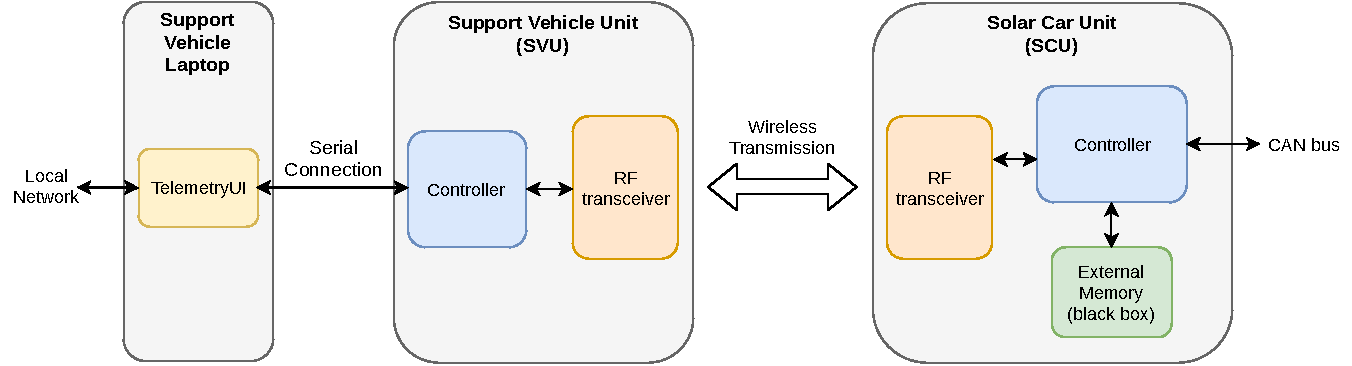
\includegraphics[width=\linewidth]{documentation/images/SystemSchematic.pdf}
    \caption{Overview of the system's components in block diagram form.}
    \label{fig:schematic}
\end{figure}

\section{Components}

\subsection{Microcontrollers} % Steffan
We use Teensy 3.6 and 4.0 microcontrollers as connection hubs in the SCU and SVU respectively. The Teensy line-up has been used as the main microcontroller platform in most DTU Roadrunners projects and we decided to use them as well after considering the performance of newer Teensy boards. Being based on the Arduino framework, both Teensys offer support for numerous protocols and software libraries to ease the implementation of our design. 

\subsection{CAN bus}
The CAN network in the SCU enables all the car's engine control units (ECU) to send and receive data without a host computer. This is possible thanks to the special structure of the CAN message.

\begin{figure}
    \centering
    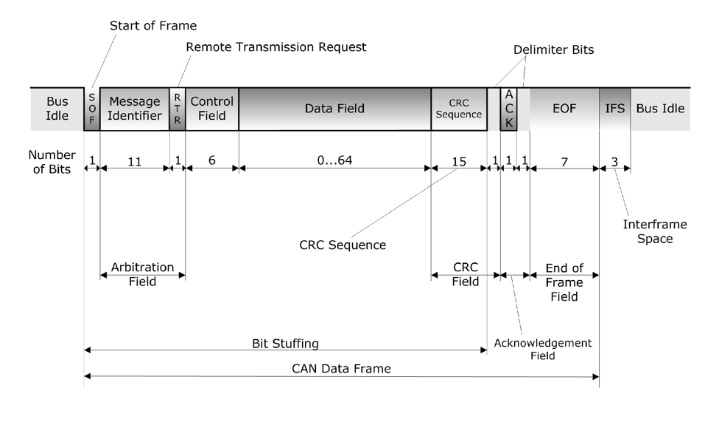
\includegraphics[width=\linewidth]{documentation/images/detailed-can-data-frame-architecture.jpg}
    \caption{Structure of a CAN frame, non-extended.}
    \label{fig:CANframe}
\end{figure}

Fig. \ref{fig:CANframe} shows a detailed structure of the CAN frame. The fields of importance for our project is the message identifier, RTR, control field and data field. The rest of the fields serve as error checking and coordination of communication on the bus.

Each ECU has a unique ID, which the message identifier uses to determine where the CAN message should go to. When two messages try to access the bus, the one with the highest priority (lowest ID) will be granted access to the bus, while the other message have to wait. After the ID comes the RTR bit which determines whether the frame remotely requests or actually sends data to a ECU. The control field, in other literature referred to as "Data Length Code" (DLC), holds the amount of bytes used in the following frame field containing the actual data\cite{DS_ISO}\cite{css}.

%The physical CAN bus itself consists of a differential pair of twisted wires, CAN High and CAN Low. These control the bits in the CAN message by setting a dominant and recessive voltage, which corresponds to a 0 and 1 respectively. A 1 is seen when the voltage in both wires is 2.5V while a 0 is seen when the CAN High wire is driven by 3.75V and the CAN Low wire is driven at 1.25V.

The Teensy 3.6 used in the solar car features a CAN controller receiving data from the CAN bus as well as handling message assembly. However, in order to interface with the physical CAN bus, a transceiver is needed. Here the MCP2551 was chosen since it has been used extensively in other DTU Roadrunners projects. The component maintains one input and one output serial stream to the CAN controller and drives the CAN bus when a message is transmitted.

\subsection{RF network} % Steffan
Two radio-frequency (RF) transceivers are required to provide a wireless connection between the SCU and SVU. There are many options for radio modules supporting long range communication at the expense of achievable data rate. We chose a trade-off between both by selecting the nRF24L01+ operating on the 2.4 GHz ISM band. The module features a detachable antenna, power amplifier and low-noise amplifier to provide a theoretical range in excess of 1000 m and data transfer rates of up to 2 Mbit/s.

An advantage of using the off-the-shelf RF module is the automated message protocol, known as Enhanced Shockburst$^\copyright$ \cite{shockburst}. Messages are transmitted in packages, structured in flexible byte segments, as shown in Fig. \ref{fig:shockburst}. Only the data payload and address needs to be specified prior to sending a package; the preamble, packet and CRC segments are generated automatically by the RF module.

\begin{figure}
    \centering
    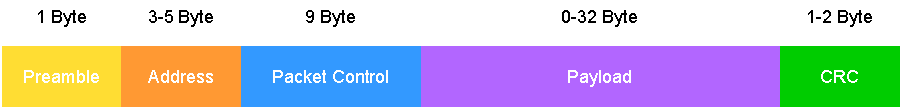
\includegraphics[width=\linewidth]{documentation/images/EnhancedShockburst.pdf}
    \caption{The Enhanced Shockburst$^\copyright$ packet structure.}
    \label{fig:shockburst}
\end{figure}

\subsection{SD card}

We chose a SD card as a permanent local storage solution for the SCU's "black box" due to its ease of use and accessibility through the Teensy 3.6 integrated SD card slot. Furthermore, this solution scales easily in terms of storage capacity, with new SD card sizes exceeding 1 TB.

\section{Software Stack}

Several key functionalities of the telemetry module are implemented in software. This, together with the aim of designing a system to be expanded upon in the future, makes the choice of software frameworks very important. Thus, an emphasis has been placed on the reusability and maintainability of the developed code.

\subsection{Build system}
As a build system, PlatformIO \cite{platformIO} was chosen for the project. It is a version control friendly, cross-platform embedded build tool which includes library management and works by defining \textit{environments} to allow development with different embedded platforms on the same code base. It comes with a VScode plugin for ideal IDE support. Other project groups working on the solar car in parallel integrated their software into the PlatformIO ecosystem as well, easing extensive code reuse in the future.

\subsection{Real Time Operating System}
We chose to build the software for the telemetry system on top of a real time operating system. The small kernel running on the microcontroller behind the scenes when using a RTOS allows a step up in abstraction from bare metal programming. Different tasks can be spawned as threads running concurrently. These threads get delegated time slots to run on the processor by the real time kernel based on their priority.

This comes at the cost of introducing overhead when switching between threads, but the great flexibility in code organization possible through the use of an RTOS was determined to make the overhead a worthwhile trade-off.

As a specific RTOS, we chose ChibiOS \cite{chibios}, since it is supported on both the Teensy 3.6 and 4.0 and because it attempts to keep the memory footprint of the real time kernel as small as possible.

\subsection{Graphical User Interface} % Tjark

The graphical user interface (GUI) included in the telemetry system serves a proof-of-concept purpose. Therefore, scala-swing \cite{scala-swing} was chosen as a framework, due to the effectiveness of the scala \cite{scala} language and the high level of abstraction used when describing a user interface in scala-swing. Furthermore, a GUI implementation in scala can run on any system with a java virtual machine and is therefore cross-platform compatible.

\subsection{Data Processing} % Steffan
Due to the wishes of DTU ROAST to use the telemetry data in applications of predictive modelling and performance optimization, we needed a way to retain the data being sent on the CAN bus, both locally via logging and remotely in real time via streaming. 

We log all the messages received on the CAN bus to the external "black box" memory as \texttt{.csv} files. Each line in the file corresponds to a message with date and time stamps, ID, RTR, DLC and 64-bit data fields as displayed in Listing \ref{lst:logFile}.

\lstset{
  basicstyle=\fontsize{9}{13}\selectfont\ttfamily
}
\begin{lstlisting}[caption={Example of a \texttt{.csv} log file with random data.},captionpos=b,label={lst:logFile}]
"time","id","rtr","len","data"
"18/06/2021 07-56-23",851,0,4,4266193389
"18/06/2021 07-56-24",55,0,6,24023809739244
"18/06/2021 07-56-24",205,0,4,3791082139
"18/06/2021 07-56-25",4,0,6,251964400399878
"18/06/2021 07-56-26",1279,0,5,65365801097
\end{lstlisting}

For remote access to the data stream we decided to implement a simple UDP network stream being hosted by the TelemetryUI. This allows all devices on the local network to monitor the data being sent over the serial connection for use in further data processing. For a POC case we created a simple Matlab script to sample CAN messages from the UDP port and print them formatted to the terminal. 

\subsection{Other Libraries}
In order to interface with the components presented in the previous section, a set of libraries were included in the project. These include a CAN network driver to support use of the Teensy 3.6's integrated CAN controller \cite{ACAN}, an RF OSI layer providing seamless integration with the nRF24L01+ modules \cite{nrfLib}, and an SD card driver to control data logging in the black box memory \cite{sdfatlib}. 

%In order to interface with the components presented in the previous section, a set of libraries were used.

%The ACAN library by Pierre Molinaro is a CAN network driver for the Teensy 3.6 board, as well as older Teensy series 3 boards. The library has been important for the connection between the CAN network and the ports on the Teensy board. We have only used the classic CAN configuration, but in addition to this, the library supports Flex CAN and CANFD. The driver supports bit rates ranging from 62.5 kbit/s up to 1 Mbit/s.

\section{Internal Communication}
The main function of the telemetry system is to bridge data streams between different end points. As such, a flexible way to pass commands and associated data payloads both ways through the system is needed. 

The majority of messages passed between the two telemetry subsystems will contain CAN messages as part of the stream from the solar car to the support vehicle. Therefore, the message protocol is designed around 16 byte messages, which are large enough to comfortably fit a CAN message and a time stamp from when the message was received. A diagram of the byte layout of a message is shown in Fig. \ref{fig:messageTypes}.

\begin{figure}
    \centering
    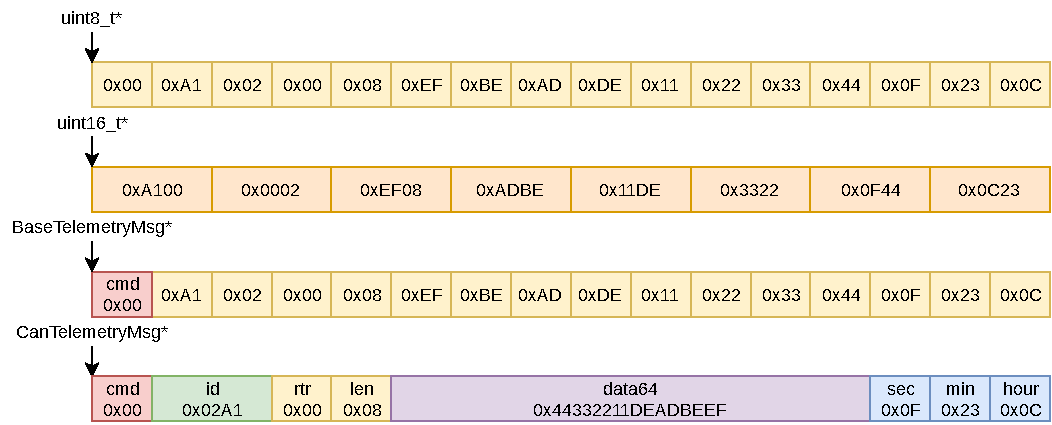
\includegraphics[width=\linewidth]{documentation/images/MessageTypes.pdf}
    \caption{The different message types used in the telemetry system.}
    \label{fig:messageTypes}
\end{figure}

The system is built around \textit{commands} and \textit{message types}. All message types begin with a command byte. The remaining 15 bytes are interpreted based on the message type. As an example, a \texttt{CanTelemetryMsg} message type is shown in Fig. \ref{fig:messageTypes}. 

One message type can be connected to different commands. For instance, the \texttt{CanTelemetryMsg} message type can be used to send data from the SCU to the SVU as part of the data stream setting the command to \texttt{RECEIVED\_CAN} = \texttt{0x00} or it can be used to inject a CAN message from the SVU into the solar car's CAN bus setting the command to \texttt{BROADCAST\_CAN} = \texttt{0x01}. Even though such message type and command combinations are only sent one direction between the telemetry modules, a unified message system for both directions was chosen due to the inherent simplicity.

When decoding messages, only the first byte needs to be considered and it will unambiguously decide how the rest of the message should be interpreted. This eases the decoding of messages on the receiving end and makes for a expandable framework. 

As an extra feature not included in our original specification, we have made an encryption protocol for our telemetry module. The feature can be activated by transmitting an \texttt{ENABLE\_ENCRYPTION} command to the SCU. The encryption is based on the RSA algorithm \cite{rsa}, which essentially generates an encryption key based on the modulus and totient function of two prime numbers. The pairings of prime numbers suited for the encryption protocol can be seen in a table uploaded to DTU ROAST BitBucket \cite{prime}. 

When a message is encrypted, each of the 16 bytes is extended to a 16-bit unsigned integer to avoid overflow problems increasing the total message size to 32 bytes. Once transmitted to the receiving node, the message is then decrypted and the overflow protection bytes can be removed leaving us with 16 bytes again. This essentially doubles the size of the data payloads being sent in our RF transmission, which is the downside of our encryption solution.

The CAN bus used in the solar car is driven at $\SI{125}{kbit/s}$. With the shortest possible CAN message being $\SI{47}{bits}$ and the longest being $\SI{111}{bits}$, a theoretical throughput of $\SI{1126}{s^{-1}}$ to $\SI{2659}{s^{-1}}$ messages can be achieved at full usage of the bandwidth.% The Teensy 3.6 being clocked at $\SI{180}{MHz}$ can thus complete between $\SI{62680}{}$ and $\SI{148016}{}$ instructions between two messages assuming it can complete one instruction per clock cycle.

The RF connection transmits Shockburst$^\copyright$ messages of worst case $\SI{392}{bits}$ length at $\SI{1}{Mbit/s}$ and is thus able to achieve a throughput of $\SI{2551}{s^{-1}}$ messages which is slightly less than the peak CAN bus throughput. This is unlikely to occur in reality, since all CAN messages need to have an empty data field to achieve the peak throughput.

A serial connection of up to $\SI{6}{Mbit/s}$ can be achieved using the Teensy 4.0. When sending from the SVU to the TelemetryUI, the message types are converted into JSON strings (see Listing \ref{lst:json}), which are worst case $\SI{117}{bytes}$ long, giving a throughput of $\SI{6410}{s^{-1}}$ messages. The JSON string can be directly used to set the state of an object inside scala which then can be used for further processing.

\lstset{
  basicstyle=\fontsize{9}{13}\selectfont\ttfamily
}
\begin{lstlisting}[caption={Example of a JSON string.},captionpos=b,label={lst:json}]
{"cmd":0,"can":{"id":1018,"rtr":false,"len":5,
"data":831599620407,
"stamp":{"hour":8,"minute":58,"second":27}}}
\end{lstlisting}

\section{Implementation}
\subsection{Solar Car Unit}

\begin{figure}
    \centering
    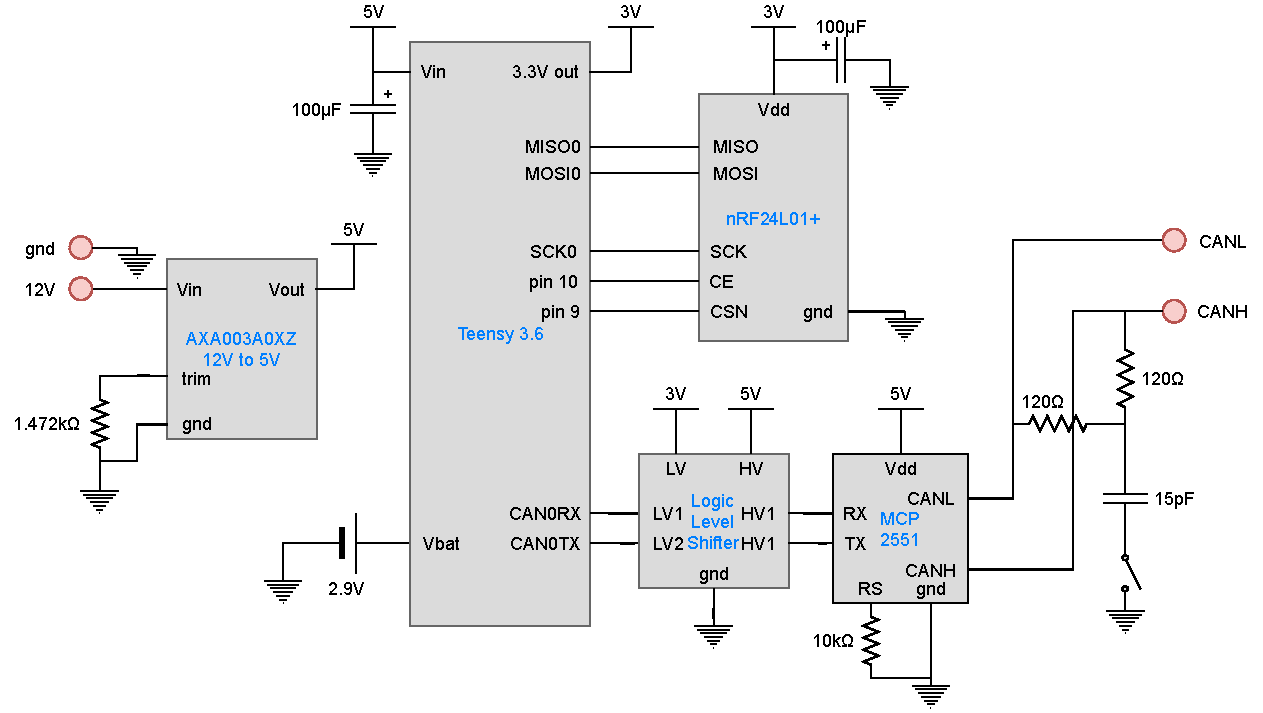
\includegraphics[width=\linewidth]{documentation/images/SCU_CircuitDiagram.pdf}
    \caption{The circuit diagram for the SCU.}
    \label{fig:SCU_circuit}
\end{figure}

The SCU is built around the Teensy 3.6 and includes the aforementioned CAN transceiver and RF module. In the solar car, all modules receive power through a molex connector at $\SI{12}{V}$. The molex connector also includes the differential pair of wires of the CAN bus. 

Different voltages are required to operate the hardware setup correctly. Therefore, a linear voltage regulator is chosen to step down the external voltage from $\SI{12}{V}$ to $\SI{5}{V}$ to power the Teensy and the CAN transceiver. The Teensy 3.6 has itself an integrated voltage regulator stepping down the input voltage to $\SI{3.3}{V}$ which we use to power the RF module.

A real time clock (RTC) is included on the Teensy 3.6 which can keep the time while the Teensy is powered off by connecting a coin cell battery to the its $V_{bat}$ terminal. This ensures that the generated time stamps associated with a received CAN message are always valid, provided the RTC is synchronized. 

A complete circuit diagram of the SCU is shown in Fig. \ref{fig:SCU_circuit}. The final circuit contains decoupling capacitors for the Teensy as well as the RF module and an optional CAN bus termination which can be activated by a switch.

\begin{figure}
    \centering
    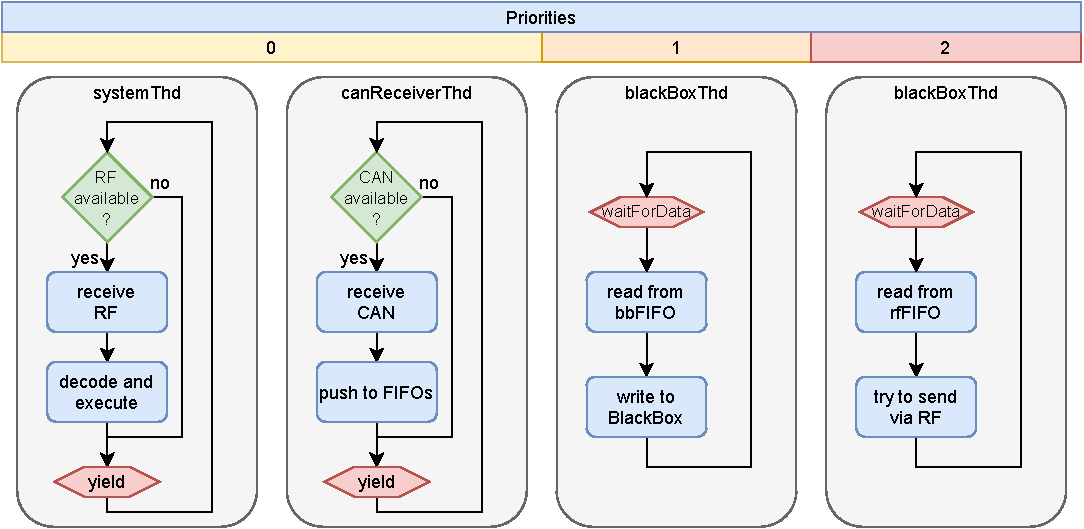
\includegraphics[width=\linewidth]{documentation/images/SCU_threads.pdf}
    \caption{The execution flow of the 4 threads running in the SCU.}
    \label{fig:SCU_threads}
\end{figure}

On the software side, the SCU is executing four threads to handle its tasks. A diagram of the execution flow of the threads is shown in Fig. \ref{fig:SCU_threads}. 

There are two threads running at the lowest priority. Since the right to execute is based on priority, these threads use a technique called \textit{cooperative multithreading} to solve the problem of arbitrating execution slots between them. Cooperative multithreading is based on the two threads voluntarily giving up their execution right by calling \texttt{yield} in reasonable time intervals, thereby giving the other thread at the same priority the right to execute \cite{chibiOsYield}.

In the system thread, messages are received via RF, decrypted, decoded and the action connected to the message is executed. The CAN receiver thread tries to receive new messages from the CAN bus. These messages then need to be passed to the two high priority threads, which process them.

This inter-thread communication is performed using two First-In-First-Out (FIFO) buffers, one for each consumer thread, which decouple the producer and the consumer. The two high priority threads only need to execute when new data is available. To achieve this, a counting semaphore is used which allows one thread to hand out execution rights by incrementing the semaphore counter and another thread to wait for execution rights \cite{chibiOsSemaphore}. This technique is used to let the producing CAN receiver thread activate the consumer threads when new data is available in the FIFO.

The black box thread takes a CAN message, converts it into a \texttt{.csv} file line and writes it into a buffer, which is emptied to the actual SD card when filled. When a predefined number of CAN messages have been logged to one file, a new file is opened. The RF thread encrypts the CAN messages and tries to send them to the SVU. If unsuccessful the RF thread goes to sleep for a predefined amount of time and wakes up periodically to reattempt transmission.

The system thread always runs in order to receive commands from the SVU. All other threads can be paused from the system thread making it easy to stop logging or streaming of the CAN data.

\subsection{Support Vehicle Unit}
The SVU is anchored around a Teensy 4.0 microcontroller connected to an RF module. The unit receives power and serial data through a micro USB cable connected to a laptop. Furthermore, the RF module is bridged via the $\SI{3.3}{V}$ supply and SPI pins. A complete circuit diagram for the SVU is shown in Fig. \ref{fig:SVU_circuit}.

On the software side, the SVU core executes two threads during operation; a \textit{receiver} thread and a \textit{transmitter} thread are both run on the same priority level with thread switching enabled by the \texttt{yield} method \cite{chibiOsYield}. The execution flow of both threads is outlined in Fig. \ref{fig:SVU_threads}. 

During execution, the receiver thread listens for incoming messages on the RF channel, decodes and relays the message to the TelemetryUI. Meanwhile, the transmitter thread waits for serial input from the TelemetryUI to transmit via the RF channel. The incoming bytes are interpreted as telemetry messages with a \texttt{cmd} field specifying the command being sent to or received from the SCU. Messages are buffered in a FIFO queue to ensure proper transmission.

\begin{figure}
    \centering
    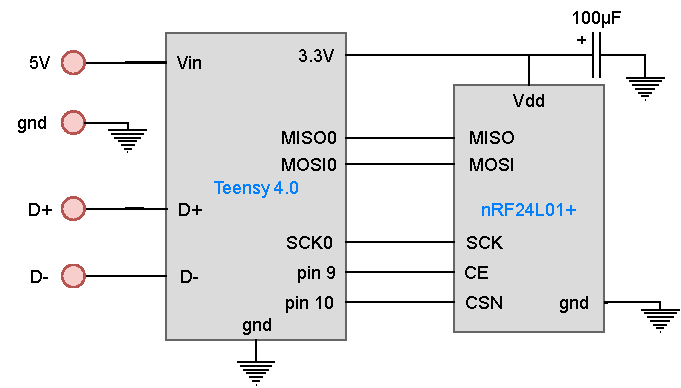
\includegraphics[width=\linewidth]{documentation/images/SVU_CircuitDiagram.pdf}
    \caption{The circuit diagram for the SVU.}
    \label{fig:SVU_circuit}
\end{figure}
\begin{figure}
    \centering
    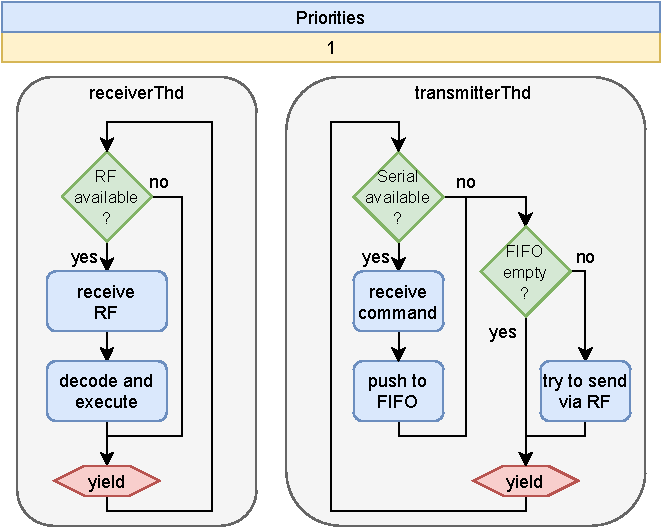
\includegraphics[height=4.5cm]{documentation/images/SVU_threads.pdf}
    \caption{The execution flow of the 2 threads running in the SVU.}
    \label{fig:SVU_threads}
\end{figure}
% threads
\subsection{TelemetryUI}

The user interface written in scala-swing is divided into three interface components: one presenting received CAN messages, one allowing the user to inject CAN messages into the solar car CAN bus, and finally one containing command buttons controlling the state of the SCU. A screenshot of the interface is shown in Fig. \ref{fig:gui_screenshot}.

In the background of the program, multithreading is used to catch new messages received via the serial connection to the SVU, which then are broadcasted to UI elements and a separate thread streaming data to the local network via a UDP port. 

\begin{figure}
    \centering
    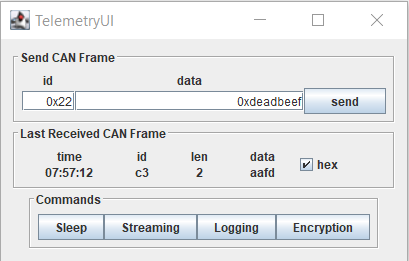
\includegraphics[width=\linewidth]{documentation/images/swing.png}
    \caption{A screenshot of the GUI.}
    \label{fig:gui_screenshot}
\end{figure}


\section{Testing and Validation} % Victor
As mentioned in the methodology section, we spent time thoroughly testing and validating our code design. Software validation was performed concurrently with writing our code to make sure that the actual behaviour of the program matched the expected behaviour. This was done through the testing environment in PlatformIO. We used this to validate our code design with unit tests, testing both edge cases and random cases.

Doing this provided us a test bench for our project, which greatly improved the credibility of our work, proving that our design works in general cases and not just the case we represent in our report.

Once all the subsystems' functionalities had been validated, testing of the final product began. Initially, we were interested in testing the efficacy of our transmission protocol by sending and receiving asynchronous messages between the SCU and SVU. Once this was demonstrated, a range test was performed in a suitable outdoor environment. In the end, we achieved a transmission range of around 160 m before the connection became too unreliable \cite{rangeTest}. 

\section{Discussion}
\subsection{Range limitation}
The measured operating range of the two RF modules turned out to be well short of the 400 m that was targeted, let alone the 1000 m claimed by the manufacturer. While this was disappointing, there are several indicators for potential range improvement. 

First of all, the hardware setup could be significantly upgraded to ensure a stable power supply to both RF modules, which seemed to be the main error source. A PCB implementation would certainly have been a possibility, given its energy-efficiency, but due to the project time frame this was not achievable. 

Secondly, time constraints prevented us in testing all of the RF module's many software configurations to enhance the range. As such, our RF modules were programmed with the default configuration and therefore not optimized for long range transmission. 

\subsection{Throughput limitation}
When testing the throughput capabilities of the system, it was found that the library code used to interface with the RF modules took up to $\SI{1200}{\mu s}$ to send one message, taking around $\SI{200000}{}$ clock cycles.

Combining the execution time spent on receiving CAN messages and writing to the black box, the SCU spent approximately $\SI{2}{ms}$ on each received CAN message, giving the system a throughput of $\SI{500}{s^{-1}}$ messages falling short of the theoretical $\SI{2659}{s^{-1}}$ messages the CAN bus can handle at peak usage by a large margin.

This shows that there is a lot of performance potential to be gained in optimizing the library code by narrowing it down to only include functionality needed for our use case. Additionally, the message protocol used internally can be optimized to reduce the number of bits sent per message, at the cost of increasing the processing workload.

One goal was to allow for automated control from the support vehicle. As for now, the CAN data stream is only broadcasted via UDP, but a UDP client can not send CAN messages the other way. Since a two way communication is already used for very basic server-client handshaking, this functionality can be integrated into the TelemetryUI relatively easily.

\section{Conclusion}
The project set out to create a telemetry module for the ROAST solar car and support car, and is successful in most of the points listed in the problem statement. The solar car module can read and write data or commands to and from the CAN bus. The solution for the processing of data in the support car uses both a GUI and streaming of data directly to Matlab. The issue of storing the data locally was solved using a SD card in the Teensy 3.6 as a black box. In addition, a feature for securely encrypting and decrypting the message was implemented.

The only features for which the final product does not meet the specification are the maximum reliable transmission distance and the maximum achievable system throughput. These issues need further enhancement in the hardware and software, which can be the basis for future projects.

However, considering all of the above, the final product still stands as a satisfactory solution to the issues listed in the problem statement.


\section*{Acknowledgment}
The authors would like to thank Martin Schoeberl and Christian Kampp Kruse for their mentoring and assistance throughout the project. The authors would also like to thank Claus Suldrup Nielsen from the department of Mechanical Engineering at DTU. 

\printbibliography

\end{document}
